\documentclass[11pt,a4paper]{report}
\usepackage{amsmath}
\usepackage{amssymb}

\usepackage{graphicx}

\usepackage{listings}
\usepackage{color} %red, green, blue, yellow, cyan, magenta, black, white
\definecolor{mygreen}{RGB}{28,172,0} % color values Red, Green, Blue
\definecolor{mylilas}{RGB}{170,55,241}


\usepackage{graphicx}


\begin{document}
\begin{center}

\LARGE Mek4250 - Mandatory assignment 2
\\
Andreas Thune
\\
\LARGE
8.05.2016

\end{center}
\textbf{Exercise 1}
\\
7.1) Given the following weak formulation of Stokes problem:
\begin{align*}
a(u,v)+b(p,v)&=(f,v) \ \forall \ v \in H_0^1(\Omega)\\
b(q,u)&=0 \ \forall q \in L^2(\Omega)
\end{align*}
Where $a(u,v) = \int_{\Omega}\nabla u : \nabla v dx$ and $b(p,v) =\int_{\Omega} p\nabla \cdot v dx$.
\\
We then want to show the following conditions required for well-posedness:
\begin{align}
&a(u,v) \leq C_1 ||u||_{H^1(\Omega)}||v||_{H^1(\Omega)} \ \forall \ v,u \in H_0^1(\Omega)\\
&a(u,u) \geq D||u||_{H^1(\Omega)}^2 \ \forall \ u \in H_0^1(\Omega)\\
&b(q,u) \leq C_2||u||_{H^1(\Omega)}||q||_{L^2(\Omega)} \ \forall \ u \in H_0^1(\Omega), \ \forall q \in L^2(\Omega)
\end{align}
Note that $u$ and $v$ are vector functions. To show the three conditions I will use the notation $u(x)=[u^1(x),...,u^d(x)]$, for $x \in  \mathbb{R}^d$. We must also remember that the inner product $":"$ in the $a$ form is defined as 
\begin{align*}
\nabla u : \nabla v = \Sigma_{i=1}^d\Sigma_{j=1}^d u_{x_j}^i(x)v_{x_j}^i(x)
\end{align*}
\\
\textbf{Inequality (1)}
\\
\begin{align*}
a(u,v)&= \int_{\Omega}\nabla u : \nabla v dx=\int_{\Omega}\sum_{i=1}^d\sum_{j=1}^d u_{x_j}^iv_{x_j}^idx \\
&=\sum_{i=1}^d\sum_{j=1}^d (u_{x_j}^i,v_{x_j}^i)_{L^2(\Omega)} \\
&\leq \sum_{i=1}^d\sum_{j=1}^d ||u_{x_j}^i||_{L^2(\Omega)}||v_{x_j}^i||_{L^2(\Omega)} \ \text{  using Cauchy-Schwartz inequality}  \\
&\leq d \sum_{i=1}^d |u^i|_{H^1(\Omega)}|v^i|_{H^1(\Omega)} \ \text{ since $||u_{x_j}^i||_{L^2} \leq |u^i|_{H^1}$} \\
&\leq d^2 |u|_{H^1(\Omega)}|v|_{H^1(\Omega)} \ \text{        using $|u^i|_{H^1} \leq |u|_{H^1}$} \\
&\leq d^2 ||u||_{H^1(\Omega)}||v||_{H^1(\Omega)} \ \text{    since $|u|_{H^1}\leq ||u||_{H^1}$ } 
\end{align*}
\\
\textbf{Inequality (2)}
\\
Using the Poincares inequality for $H_0^1(\Omega)$, given by: 
\begin{align*}
|u|_{H^1(\Omega)}^2\geq C||u||_{L^2(\Omega)}^2
\end{align*} 
we get 
\begin{align*}
a(u,u)&= \int_{\Omega}\nabla u : \nabla u dx=\int_{\Omega}\sum_{i=1}^d\sum_{j=1}^d u_{x_j}^iu_{x_j}^idx \\
&=\sum_{i=1}^d\sum_{j=1}^d ||u_{x_j}^i||_{L^2(\Omega)}^2=\sum_{i=1}^d |u^i|_{H^1(\Omega)}^2 = |u|_{H^1(\Omega)}^2 \\
&= \frac{1}{2}(|u|_{H^1(\Omega)}^2+|u|_{H^1(\Omega)}^2) \\
&\geq \frac{1}{2}(|u|_{H^1(\Omega)}^2+C||u||_{L^2(\Omega)}^2) \\
&\geq \frac{min\{1,C\}}{2}(|u|_{H^1(\Omega)}^2+||u||_{L^2(\Omega)}^2) \\
&= D||u||_{H^1(\Omega)}^2
\end{align*}
\\
\textbf{Inequality (3)}
\\
\begin{align*}
b(q,u)&=\int_{\Omega} q\nabla \cdot u dx=\int_{\Omega}\sum_{i=1}^d qu_{x_i}^i dx \\
&\leq \sum_{i=1}^d ||q||_{L^2(\Omega)} ||u_{x_i}^i||_{L^2(\Omega)} \ \text{  using Cauchy-Schwartz inequality}  \\
&\leq ||q||_{L^2(\Omega)}\sum_{i=1}^d |u^i|_{H^1(\Omega)} \\
&\leq d||q||_{L^2(\Omega)}|u|_{H^1(\Omega)} \\
&\leq d||q||_{L^2(\Omega)}||u||_{H^1(\Omega)}
\end{align*}
\\
7.6) Want to solve the the stokes problem with a manufactured solution $ue(x,y)=(\sin(\pi y),\cos(\pi x))$ and $pe(x,y)=\sin2\pi x)$ on $\Omega = (0,1)^2$. This means solving the problem:
\begin{align*}
-\Delta u - \nabla p &= f \\
\nabla \cdot u &= 0 \\
u &= ue \ \text{on } \partial\Omega_D \\
-\frac{\partial u}{\partial n} - pn &= h \ \text{on } \partial\Omega_N
\end{align*} 
To be able to solve the equation we need to define $\partial\Omega_D$ and $\partial\Omega_N$, as well as deriving $f$ and $h$. 7.7 use $\partial\Omega_N= \{y=0\}$ and $\partial\Omega_D=\partial\Omega - \partial\Omega_N$. This gives us $h=(-\pi,-sin(2\pi x))$. We see this by noting that $n=(0,-1)$ on $\partial\Omega_N$, and calculating:
\begin{align*}
h &= -\frac{\partial u(x,0)}{\partial n} - p(x,0)n  = -(\nabla u_1\cdot n,\nabla u_2\cdot n) -\sin(2\pi x)n\\
&= -( [0,\pi \cos(\pi \cdot0)] \cdot[0,-1], ( [-\pi \sin(\pi x),0]\cdot[0,-1]) +(0,-\sin(2\pi x)) \\
& = (-\pi,0)+(0,-\sin(2\pi x)) = (-\pi,-\sin(2\pi x))
\end{align*}
Now lets find $f$:
\begin{align*}
f &= -\Delta u - \nabla p \\
&= (\pi^2 \sin(\pi y),\pi^2 \cos(\pi x)) - (2\pi\cos(2\pi x),0) 
\end{align*} 
The last step before implementing the numerics is to derive the variational form:
\begin{align*}
-\int_{\Omega} \Delta u \cdot v  dx - \int_{\Omega} \nabla p \cdot v  dx &= \int_{\Omega} \nabla u :\nabla v  dx + \int_{\Omega} p \nabla\cdot v  dx -\int_{\partial\Omega_n}(\frac{\partial u}{\partial N} + pn)\cdot v  dS \\
&=\int_{\Omega} \nabla u :\nabla v  dx + \int_{\Omega} p \nabla\cdot v  dx +\int_{\partial\Omega_N}h\cdot v  dS 
\end{align*}
Together with the deivergence term this gives us the following variational form:
\begin{align*}
\int_{\Omega} \nabla u :\nabla v \ dx + \int_{\Omega} p \nabla\cdot v \ dx +\int_{\Omega} q\nabla\cdot u  \ dx = \int_{\Omega} f\cdot v \ dx +\int_{\partial\Omega_N}h\cdot v \ dS 
\end{align*}
As usual this should hold $\forall$ $v \in H_0^1(\Omega)\times H_0^1(\Omega)$ and $\forall$ $q \in L^2(\Omega)$. We also deal with the Dirichlet boundary condition in the normal way (ignoring them, and fixing the system). 
\\
\\
The FEniCS implementation of this problem using the four combinations of elements asked for in the exercise is added at the end of the assignment. We were then asked to test if our approximations converged at the expected rate. The natural way of measuring the error is using $H^1$ norm for velocity and $L^2$ norm for pressure. The theoretical convergence rate is then given by the following inequality:
\begin{align*}
||u-u_h||_{H^1}+||p-p_h||_{L^2} \leq Ch^{q}||u||_{H^{q+1}}+Dh^{t+1}||p||_{H^{t+1}}
\end{align*}
Here $q$ and $t$ are the degrees of the elements used in our finite element spaces. Using $h=\{\frac{1}{8},\frac{1}{16}, \frac{1}{32},\frac{1}{64}\}$ I got the following results using least squares:
\begin{center}
    \begin{tabular}{| l | l | l |}
    \hline
     & Convergence rate & Constant  \\ \hline
    $P4-P3$ & 4.045257 & 0.084663 \\ \hline
    $P4-P2$ & 2.902867 &  0.493978	\\ \hline
    $P3-P2$ & 2.890269 & 0.447429\\ \hline
    $P3-P1$ & 2.024947 &  1.135217	\\ \hline
    \end{tabular}
\end{center}
I justify using least squares by doing a loglog plot of the error and the mesh resolution for the different element types. We see that the loglog plot is straight lines for all elements, and using least squares therefore makes sense.
\begin{figure}
  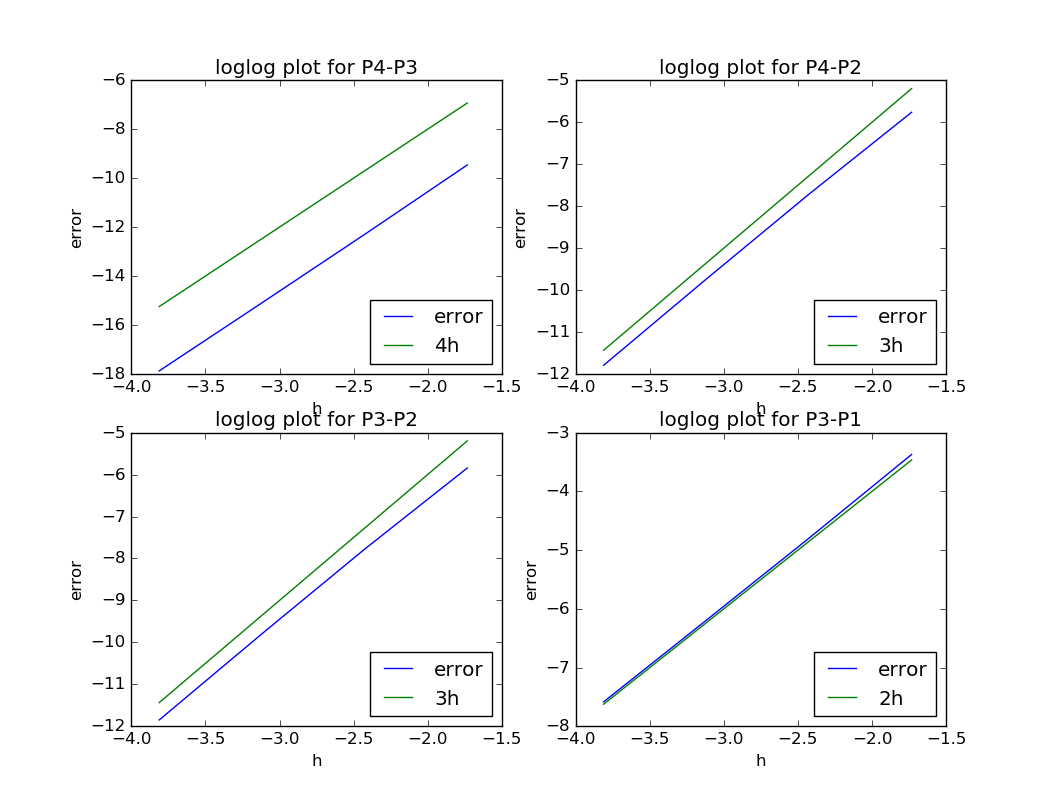
\includegraphics[width=\linewidth]{element_con.png}
  \caption{loglog plot for the error plotted together with linear functions with the expected steepness. Observe that the slope of the expected line and the error plot are almost the same for all element combos}
  \label{Fig 1}
\end{figure}
\\
\\
7.7) The wall shear stress is defined in the exercise. Defining \\$\Gamma = \{(x,y) \in \Omega | x=0 \}$, and the unit vector $t=[0,1]$ parallel to $\Gamma$, the wall shear stress is defined as: 
\begin{align*}
||\nabla u\cdot t||_{L^2(\Gamma)}^2 &= \int_{\Gamma} |\nabla u \cdot t|^2  \ dS \\
&=  \int_{\Gamma} |(\nabla u_1 \cdot t,\nabla u_2 \cdot t)|^2  \ dS \\
&=\int_{\Gamma} \frac{\partial u_1}{\partial y}^2 + \frac{\partial u_2}{\partial y}^2 \ dS
\end{align*} 
Using this I calculated the convergence rate for different element combos, by solving the equation for the same mesh resolutions as in 7.6. To calculate the convergence rates I used least squares, and the results were as follows:
\begin{center}
    \begin{tabular}{| l | l | l |}
    \hline
     & Convergence rate & Constant   \\ \hline
    $P4-P3$ & 3.999511 & 0.011619    \\ \hline
    $P4-P2$ & 3.999512 & 0.011619	\\ \hline
    $P3-P2$ & 2.999236 & 0.077591    \\ \hline
    $P3-P1$ & 2.999236 & 0.077591	\\ \hline
    	$P4-P1$ & 3.999512 & 0.011619	\\ \hline
    \end{tabular}
\end{center}
These results seems to indicate the following convergence result for wall shear stress:
\begin{align*}
||\nabla (u-u_h)\cdot t||_{L^2(\Gamma)} \leq Ch^q
\end{align*} 
Where $q$ is equal to the degree of the element used for velocity, and the both constant $C$ and $q$ is independent of the pressure element. I solved the equation using $P4-P1$ elements to show that this relation also holds for element combos where the diffrence in degree is bigger then $2$. As in exercise 7.6 I have added a loglog plot to justify use of least squares.
\begin{figure}
  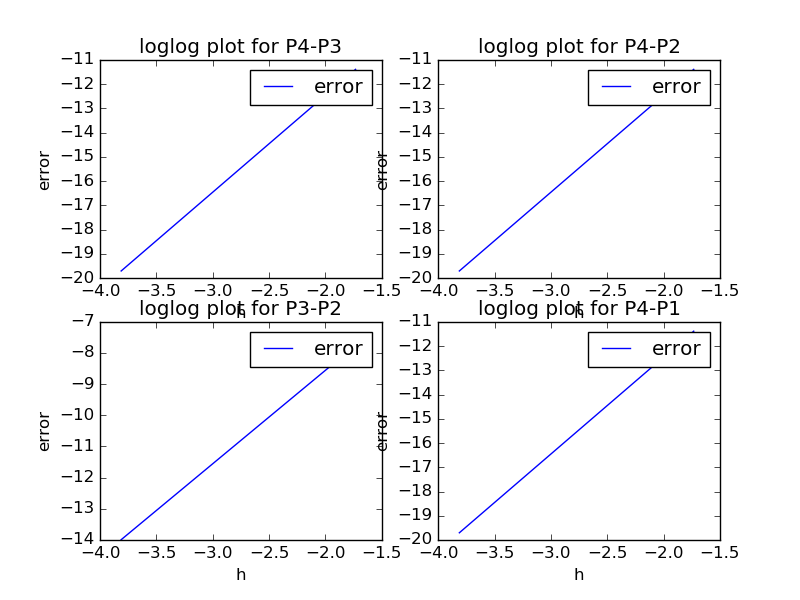
\includegraphics[width=\linewidth]{stress_con.png}
  \caption{loglog plot for the wall shear stress error $||\nabla (u-u_h)\cdot t||_{L^2(\Gamma)}$. Observe that lines are almost linear.}
  \label{Fig 2}
\end{figure}
\end{document}